
\begin{enumerate}
    \item Solving first pair of inequality:
    \begin{align}
\label{ineq/56/eq:line_one_ineq}
\begin{split}
    -x+2y &\geq -3
\\
    3x+4y &\geq 12
\end{split}
\end{align}
\solution  Let $u_1 \ge 0, u_2 \ge 0$.  This may be expressed as
\begin{align}
\vec{u} = \myvec{u_1\\u_2}\succeq \vec{0}
\end{align}
%
\eqref{ineq/56/eq:line_one_ineq} can then be expressed as
\begin{align}
\myvec{-1 & 2 \\ 3 & 4}\vec{x}  &\succeq \myvec{-3\\12}
\\
\myvec{-1 & 2 \\ 3 & 4}\vec{x}  -\vec{u}&=\myvec{-3\\12}
\\
\text{or, }
\myvec{-1 & 2 \\ 3 & 4}\vec{x} &= \myvec{-3\\12} +\vec{u}
\end{align}
%
resulting in 
\begin{align}
\vec{x} &= \myvec{-1 & 2 \\ 3 & 4}^{-1}\myvec{-3\\12} +\myvec{-1 & 2 \\ 3 & 4}^{-1}\vec{u}
\\
\text{or, } \vec{x} &= \myvec{3.6\\0.3} +\frac{-1}{10}\myvec{4 & -2 \\ -3 & -1}\vec{u}\label{ineq/56/eq:1}
\end{align}
    
    \item Similarly,Solving second pair of inequality:
    \begin{align}
\label{ineq/56/eq:line_two_ineq}
\begin{split}
    x\geq 0
\\
    y \geq 1
\end{split}
\end{align}
\solution  Let $u_1 \ge 0, u_2 \ge 0$.  This may be expressed as
\begin{align}
\vec{u} = \myvec{u_1\\u_2}\succeq \vec{0}
\end{align}
%
\eqref{ineq/56/eq:line_two_ineq} can then be expressed as
\begin{align}
\myvec{1 & 0 \\ 0 & 1}\vec{x}  &\succeq \myvec{0\\1}
\\
\myvec{1 & 0 \\ 0 & 1}\vec{x}  -\vec{u}&=\myvec{0\\1}
\\
\text{or, }
\vec{x} &= \myvec{0\\1} +\vec{u}\label{ineq/56/eq:2}
\end{align}
\end{enumerate}
From \eqref{ineq/56/eq:1} and \eqref{ineq/56/eq:2},solution of the given system of inequalities can be found out graphically by intersection as shown by the below figures generated by Python:
As seen from Fig. \ref{ineq/56/fig:inequality3} the solution region is bounded by line segments AB and BC and the line $\myvec{1&-2}\vec{x}=3$.Beyond A the region expands infinitely along the Y axis,Beyond C the region includes all the portion above the line $\myvec{1&-2}\vec{x}=3$.


\begin{figure}[!ht]
    \centering
    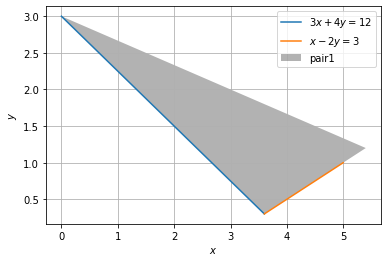
\includegraphics[width=\columnwidth]{solutions/su2021/2/56/Figure9_1.png}
    \caption{Inequality pair 1}
    \label{ineq/56/fig:inequalities1}	
    \end{figure}
    
    \begin{figure}[!ht]
    \centering
    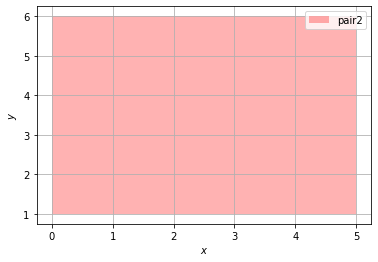
\includegraphics[width=\columnwidth]{solutions/su2021/2/56/Figure9_2.png}
    \caption{Inequality pair 2}
    \label{ineq/56/fig:inequalities2}	
    \end{figure}
    
    \begin{figure}[!ht]
    \centering
    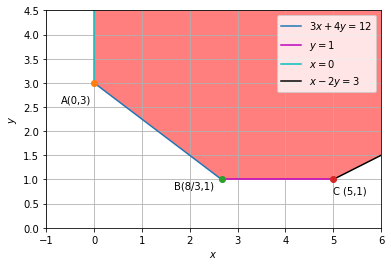
\includegraphics[width=\columnwidth]{solutions/su2021/2/56/Figure 9_3.png}
    \caption{Intersection of \ref{ineq/56/fig:inequalities1} and \ref{ineq/56/fig:inequalities2}}
    \label{ineq/56/fig:inequality3}	
    \end{figure}
    The common region shown by \ref{ineq/56/fig:inequality3} is the solution of set of inequalities.
    